\cchapter{مروری بر ادبیات}
در این بخش سعی داریم تا با مروری بر اصطلاحات و ابزارهای مورد استفاده در پژوهش‌های بررسی شده، با پیش‌نیازهای مبحث موردنظر آشنا شویم. 

\section{DRX/DTX}

\begin{figure}
	\centering
	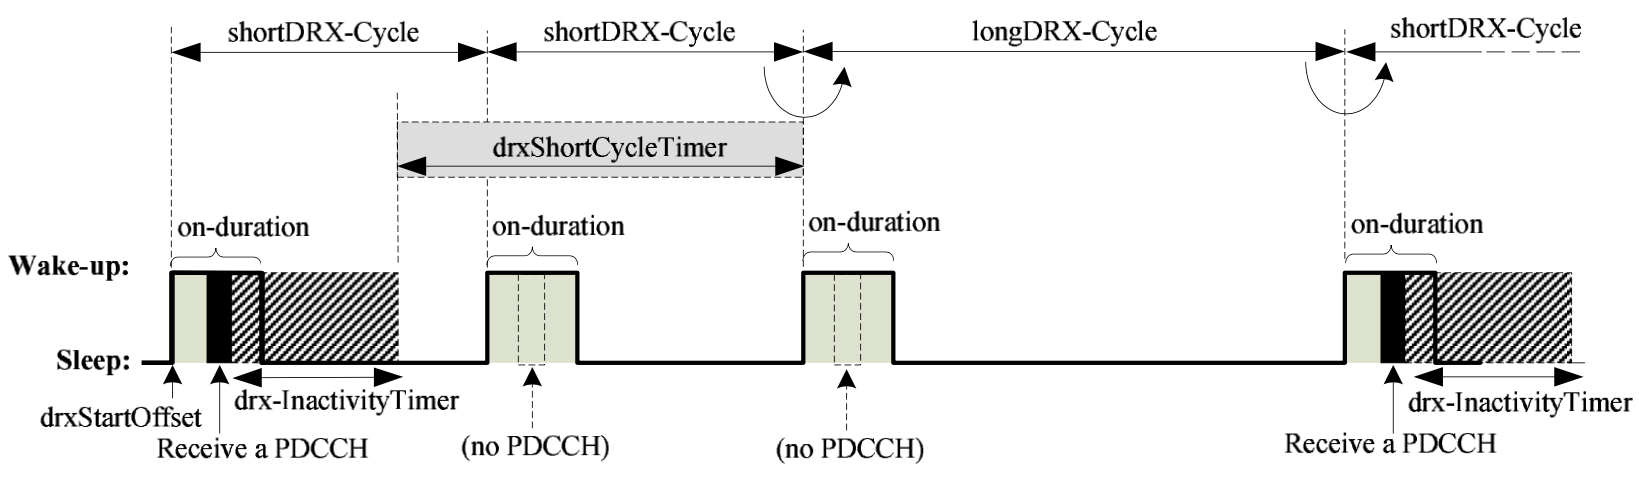
\includegraphics[width=\linewidth]{figs/drx}
	\caption {شمای فعالیت مکانیزم DRX/DTX}
	\label{fig:drx}
\end{figure}

\lr{Discontinuous Reception/Transmission}
یا به اختصار 
\lr{DRX/DTX}
یک مکانیزم از پیش تعریف شده بر بستر شبکه‌های بی‌سیم است که به کمک آن می‌توان زمانبندی فعالیت هر یک از اعضای شبکه (که به اصطلاح، به آن گره\LTRfootnote{Node} نیز گفته می‌شود) ساماندهی نمود. همان‌گونه که در شکل \ref{fig:drx} مشاهده می‌نمایید؛ در شبکه‌هایی که از این مکانیزم استفاده می‌شود در واقع یک چهارچوب خاص برای فعالیت گره‌ها وجود دارد و رفتار ثابت و ازپیش‌تعریف‌شده‌ای را از گره‌ها شاهد هستیم. اما آن‌چه تفاوت در میان گره‌هارا رقم می‌زند مقادیر پارامترهایی است که در این مکانیزم به کار می‌روند. پارامتر‌های \lr{DRX/DTX} هر یک، بیانگر زمان مورد نیاز برای یک رویداد در رفتار گره‌ها هستند. در ادامه به توضیح هر یک از این پارامتر‌ها می‌پردازیم.

\subsection{drxStartOffset}
این پارامتر بیانگر \lr{Offset} زمانی اولیه‌ی پیش از شروع فرآیند توسط گره‌ی شبکه می‌باشد. بدیهی است که تا پیش از این زمان، گره هنوز فعالیت خود را آغاز نکرده است.

\subsection{on-duration}
این پارامتر نمایان‌گر مدت زمانی‌است که پس از هر بار فعال شدن، گره فعال می‌ماند و در انتظار دریافت داده از سایر گره‌ها می‌باشد. گفتنی‌ست که این مدت زمان فعال ماندن یک گره برحسب نیاز می‌تواند افزایش یابد که در ادامه به آن خواهیم پرداخت.

\subsection{drx-InactivityTimer}
پیش‌تر گفتیم که یک گره‌ی شبکه، در زمان خاصی از حالت غیرفعال خارج شده و در انتظار دریافت داده از سایر گره‌های موجود در شبکه می‌ماند. این زمان، در واقع همان زمانی است که در بخش پیش به تعریف آن پرداختیم. اما در آنجا نیز اشاره شد که در صورت دریافت سیگنال از سایر گره‌ها، نیازمند زمان فعالیت بیشتری برای گره هستیم. دلیل آن نیز واضح است. چرا که اگر در اواخر زمان \lr{on-duration}، بسته‌ای (سیگنالی) توسط گره‌ی مذکور دریافت شود، طبیعتا پردازش و در صورت نیاز، پاسخ‌دهی به آن نیازمند زمان است. پس طبق آن‌چه از مرور چنین شرایطی درک می‌نماییم؛ پس از دریافت یک سیگنال، گره نیازمند است تا زمان اضافه‌تری برای فعالیت در اختیار داشته باشد که این زمان اضافه را، \lr{drx-InactivityTimer} می‌نامند. لازم به ذکر است که در این زمان، همان‌طور که از نام این پارامتر نیز مشهود است؛ گره امکان پاسخگویی به درخواست دیگری را ندارد.

\subsection{shortDRX-Cycle}
تمام فرآیندهای ذکر شده در بخش‌های بالا، در یک تناوب مشخصی تکرار می‌شوند که پارامتر \lr{shortDRX-Cycle} بیان‌گر مدت زمان یک دوره می‌باشد. همان‌طور که در شکل \ref{fig:drx} نیز مشاهده می‌شود، طول دوره، به از زمان پارامتر \lr{on-duration} بیشتر خواهد بود. چرا که در هر دوره گره پس از شروع شدن زمان فعالیت، مدتی را منتظر دریافت سیگنال از جانب سایر گره‌ها می‌ماند. پس از این زمان، گره باید قادر باشد تا مدتی را غیرفعال گردد و میزان مصرف انرژی سیستم را کاهش دهد. از این رو، بدیهی است که مدت زمان دوره از زمان فعالیت دستگاه طولانی‌تر باشد.

\subsection{longDRX-Cycle}
پیش از این با مفهوم دوره در شبکه‌های مبتنی بر مکانیزم \lr{DRX/DTX} آشنا شدیم. اما یکی دیگر از جنبه‌های قابل توجه در این مکانیزم، وجود دوره با دو مدت زمان متفاوت است. در این مکانیزم، دو دوره با مدت‌ زمان‌های کوتاه و بلند وجود دارد. فعالیت دستگاه در این سیستم‌ها با دوره کوتاه آغاز می‌شود اما در صورتی که مدتی دستگاه پس از فعال شدن و انتظار دریافت سیگنال، هیچ سیگنالی دریافت نکند؛ در این شرایط وارد دوره‌های بلند مدت می‌شود. از آن‌جا که تمامی پارامتر‌های ذکر شده در بالا برای هر دو طول دوره یکسان است، می‌توان نتیجه گرفت که دوره طولانی‌تر به مدت زمان غیرفعال بودن طولانی‌تری برای دستگاه می‌انجامد و به همین ترتیب میزان مصرف انرژی گره بیش از پیش کاهش می‌یابد.

\subsection{drxShortCycleTimer}
این پارامتر بیانگر مدت زمانی است که پس از آن، دستگاه از دوره‌های کوتاه مدت وارد دوره‌های بلند مدت می‌شود تا انرژی کمتری مصرف نماید.

\begin{figure}
	\centering
	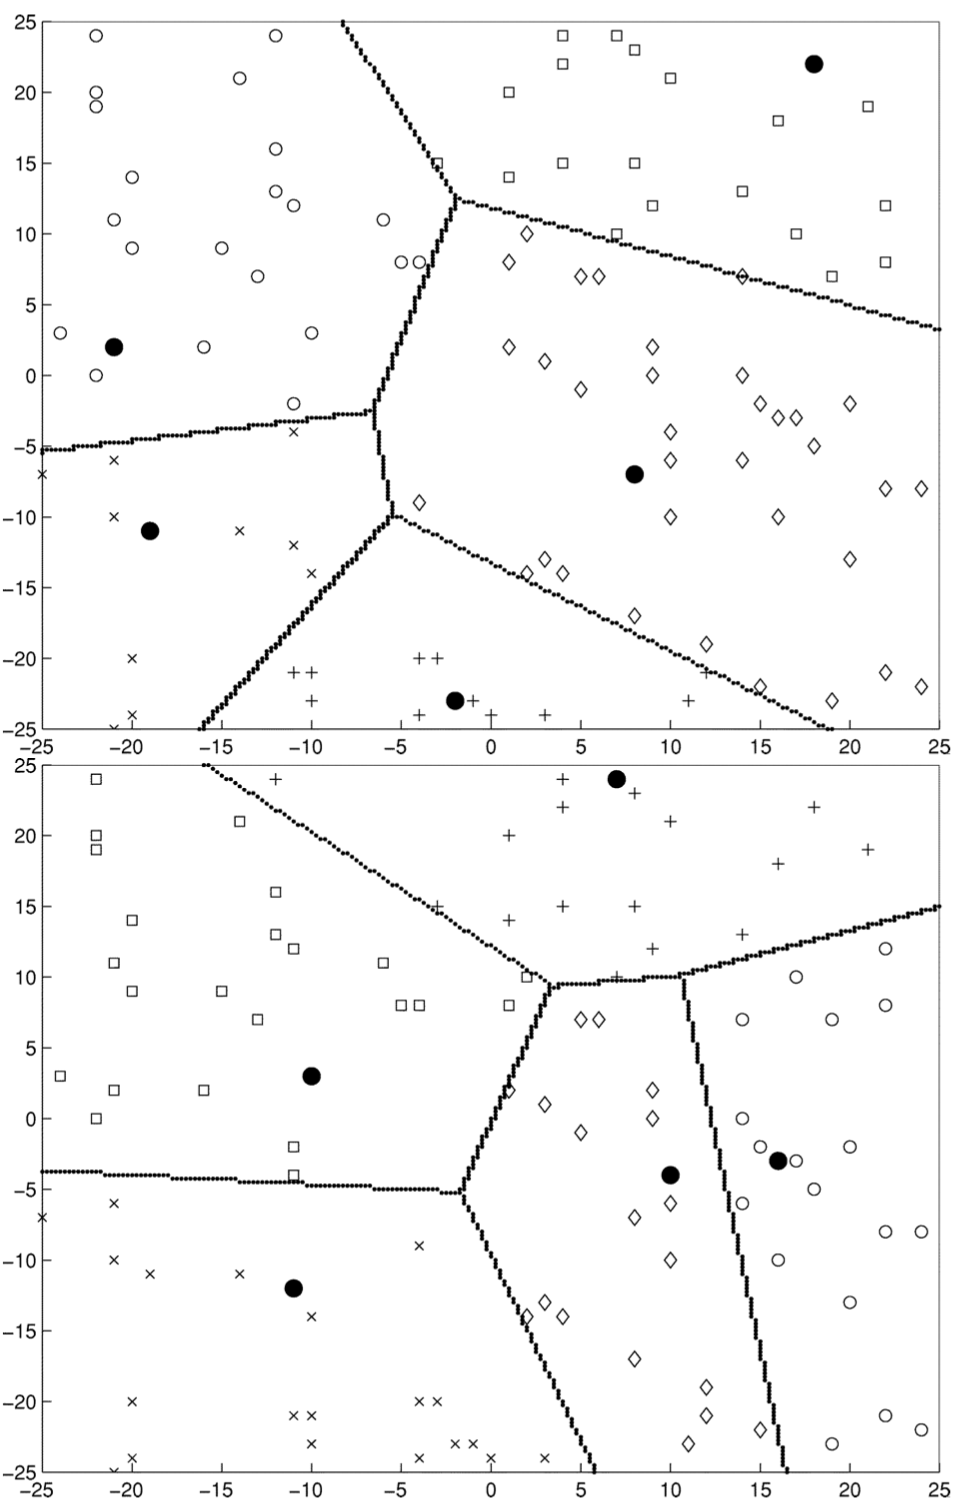
\includegraphics[width=0.7\linewidth]{figs/leach}
	\caption {انتخاب گره‌ی سرگروه و خوشه‌بندی در دو بازه‌ی زمانی متفاوت توسط الگوریتم LEACH}
	\label{fig:leach}
\end{figure}

\section{LEACH}
در مبحث کارهای صورت‌گرفته، در ادامه خواهیم دید که یکی از رویکردها جهت کاهش مصرف منابع انرژی توسط حسگرها در سیستم‌های مبتنی بر رایانش ابری، ارائه گراف یا توپولوژی‌ای برای مشخص نمودن حالت بهینه‌ی ارتباط میان اجزا می‌باشد. در این رویکردها یکی از تکنیک‌های به کار برده شده این است که به دلیل ساختار سلسله‌مراتبی‌شان، در هر حالت، گره‌ای به عنوان گره اصلی خوشه\LTRfootnote{Head node} انتخاب می‌گردد. به طور خلاصه اگر به بیان وظیفه این گره نگاه کنیم؛ در واقع این گره مسئولیت انتقال داده از سطوح بالاتر همچون \lr{Base Station} به حسگرها و همچنین جمع‌آوری داده‌ها از حسگرها و ارسال مجدد آن‌ها برای \lr{Base Station} را بر عهده دارد.
\par
در چنین شرایطی بدیهی است که گره‌ای که به عنوان گره سرگروه خوشه انتخاب می‌گردد؛ دارای فعالیت ارتباطی بیشتری با سایر گره‌ها دارد و در نتیجه منابع انرژی بیشتری را نسبت به سایر گره‌ها مصرف می‌نماید. حال اگر فرض کنیم فرآیند انتخاب گره سرگروه یک فرآیند ثابت باشد - یعنی فقط یک بار گره‌ای را به عنوان سرگروه مشخص کنیم و دیگر آن را تغییر ندهیم - آن‌چه به وقوع می‌پیوندد، این است که در هر خوشه یا منطقه‌ای که مستقلا به عنوان یک گروه در نظر گرفته شده است، یک گره (که همان گره سرگروه است) با مصرف حداکثری انرژی به کار خود ادامه ‌می‌دهد تا زمانی که منابع انرژی خود را به طور کامل مصرف کرده و خاموش گردد. در این رویکرد همان‌طور که قابل مشاهده است، طول عمر سیستم کاهش می‌یابد و این دقیقا در تناقض با یکی از اهداف اصلی ما، یعنی افزایش طول عمر سیستم است.
\par
به همین منظور، الگوریتمی که در مقاله \cite{} معرفی شده است، الگوریتم \lr{LEACH} (مخفف‌شده‌ی عبارت: \lr{Low-Energy Adaptive Clustering Hierarchy}) می‌باشد. رویکرد این الگوریتم به این صورت است که به صورت دوره‌ای، گره سرگروه هر خوشه را تغییر می‌دهد تا سربار انرژی حاصل از برقراری ارتباط میان اجزای سیستم، به طور متوازن میان تمامی گره‌های عضو خوشه تقسیم گردد و در نتیجه، به افزایش طول عمر سیستم منجر شود. در شکل \ref{fig:leach} نمونه ای از رفتار این الگوریتم را در دو دوره‌ی متفاوت زمانی مشاهده می‌کنید.

\section{انواع حسگرها}
همان‌طور که می‌دانیم؛ حسگرهای به کار رفته در یک سیستم مبتنی بر اینترنت اشیا، عمدتا مسئولیت مشاهده و دریافت اطلاعات از محیط را بر عهده دارند و این امر به واسطه‌ی ارتباطشان با \lr{Base Station} و کوئری درخواست شده از جانب آن صورت می‌گیرد. بر این اساس، حسگرهای مبتنی بر اینترنت اشیا، از لحاظ رفتار و نحوه فعالیتشان به دو دسته اساسی تقسیم می‌شوند. این دو دسته عبارتند از:
\begin{itemize}
	\item{حسگرهای Trigger-Based}
	\item{حسگرهای Periodic}
\end{itemize}
\par
در ادامه به تشریح هر یک از انواع مذکور می‌پردازیم.

\subsection{حسگرهای Trigger-Based}
دسته‌ی اول حسگرهای موجود در سیستم‌های مبتنی بر اینترنت اشیا، حسگرهایی هستند که بر اساس یک رویداد خاص در محیط فعال شده و به مشاهده محیط پیرامون می‌پردازند. برای مثال؛ حسگرهای حرکتی از این دست هستند و از کاربردهای مرتبط با آن‌، می‌توان به سیستم‌های روشنایی خودکار محیط اشاره کرد. در این سیستم‌ها با ایجاد حرکت در محیط، حسگر فعال می‌شود و سیگنالی را به \lr{Base Station} تا کنترل‌کننده\LTRfootnote{Controller} سیستم، دستور روشن شدن چراغ‌های موجود در محیط را ارسال کرده و روشنایی محیط تامین شود.

\subsection{حسگر‌های Periodic}
دسته دیگر حسگرهای موجود در سیستم‌های مبتنی بر اینترنت اشیا، حسگر‌های \lr{Periodic} هستند. این حسگرها، فعالیتشان منوط به یک رویداد خاص در محیط نیست و به طور مداوم در حال پایش و مشاهده محیط هستند. برای مثال حسگرهای دمای محیط اغلب به صورت \lr{Periodic} فعالیت می‌کنند. چرا که تغییرات دما در یک محیط عمدتا به صورت پیوسته بوده و همواره در جریان است. اما به این دلیل می‌گوییم اغلب، چرا که حسگر‌های دما نیز می‌توانند به صورت \lr{Trigger-Based} فعالیت کنند و برای مثال؛ صرفا بر اساس تجاوز دما از یک درجه‌ی خاص و یا کاهش دما به میزانی کمتر از حد معین، سیگنال موردنظر را به \lr{Base Station} مخابره نماید تا سیستم، تغییرات خود را بر محیط اعمال کند.

\par
بدیهی است که در یک سیستم مبتنی بر اینترنت اشیا، هر دو نوع حسگرها می‌توانند در کنار یکدیگر به فعالیت بپردازند. یک مثال معروف در این زمینه که در مقاله \cite{} آمده است، مثال مدیری است که برای جلسه فردا برنامه‌ریزی می‌کند. در این مثال بیان می‌شود که یک مدیر، برای جلسه فردای خود که در ساعت هشت صبح است ساعتش را کوک می‌کند تا در ساعت ۷ صبح بیدار شود. در این بین، در ساعت ۶:۳۰ صبح گوشی مدیر با چک کردن داده‌های مربوط به ترافیک متوجه ترافیک سنگین می‌شود و مدیر را زودتر بیدار می‌کند. پنج دقیقه بعد، زمانی که مدیر در حال استحمام است؛ سیستم، دستور فعال شدن را برای دستگاه چای‌ساز صادر می‌کند تا در هنگام آماده شدن مدیر چای، آماده باشد و چای‌ساز در زمانی که چای آماده می‌شود، سیگنالی را به سیستم میفرستد تا سیستم از این رویداد آگاه گردد. در این همین مثال مشاهده می‌شود که هر دو نوع حسگرهای \lr{Trigger-Based} و \lr{Periodic} در حال فعالیت در کنار یکدیگر می‌باشند. برای مثال؛ حسگر موجود در دستگاه چای‌ساز به صورت \lr{Trigger-Based} عمل می‌نماید. حال آن‌که گوشی - که به عنوان حسگر ترافیک در سیستم مشغول به کار است - به صورت \lr{Periodic} فعال است. نکته دیگر در تفاوت میان این دو نوع حسگر این است که به طور معمول، حسگرهای \lr{Periodic} اطلاعات کاملی را از محیط مورد پایش خود به کنترل‌کننده ارائه می‌کنند. در صورتی که در اغلب موارد، حسگرهای \lr{Trigger-Based} صرفا یک سیگنال را که بیانگر وقوع رویداد است مخابره می‌کنند و این سیگنال شامل پارامترهای اضافی نیست.

\section{خودسازماندهی}
یکی از مفاهیم به کار رفته در مقاله \cite{} که در فصل بعدی به تفصیل به آن خواهیم پرداخت، خودسازماندهی\LTRfootnote{Self-Configuration} است. خودسازمندهی به معنی توانایی سیستم به ایجاد تغییر در رفتار خود به منظور بهبود عملکرد سیستم بوده و شامل جنبه‌های گوناگونی است که در ادامه به توضیح مختصری از هر یک می‌پردازیم. لازم به ذکر است؛ تعاریف ارائه شده در مقاله مذکور هیچ یک به تنهایی چرخه \lr{MAPE} را به وجود نمی‌آورند. اما از مجموعه این اعمال چرخه\lr{MAPE} پدید خواهد آمد. چرخه \lr{MAPE} یک چرخه تکاملی است که در سیستم‌های خودسازمانده وجود دارد و حرکت سیستم در راستای این چرخه منجر به خودمختاری سیستم می‌گردد. این چرخه شامل چهار مرحله زیر است. در شکل \ref{fig:mape} می‌توانید این چرخه را مشاهده نمایید. 
\begin{itemize}
	\item{$Monitoring$ به معنی مشاهده و پایش محیط و دریافت اطلاعات از آن.}
	\item{$Analayze$ به معنی دریافت اطلاعات و پردازش آن‌ها که منجر به درک سیستم از محیط می‌گردد.}
	\item{$Planning$ به معنی تصمیم‌گیری برای ایجاد تغییرات بر روی محیط براساس دانش موجود در ارتباط آن.}
	\item{$Execution$ اعمال تغییرات برنامه ریزی شده در مرحله قبلی براساس ارسال دستورات به عمل‌کننده‌های محیطی.}
\end{itemize}
\par
در مقاله مذکور سه اصل جهت ایجاد چنین چرخه‌ای ذکر شده است که این مراحل به شرح زیر ‌می‌باشند.
\begin{itemize}
	\item{خودپیکربندی\LTRfootnote{Self-Configuration}}
	\item{خودبهینگی\LTRfootnote{Self-Optimization}}
	\item{خودالتیامی\LTRfootnote{Self-Healing}}
\end{itemize}

\begin{figure}
	\centering
	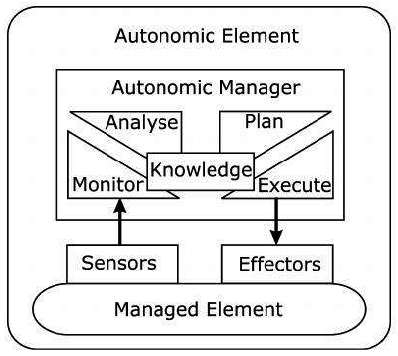
\includegraphics[width=0.5\linewidth]{figs/mape}
	\caption {چرخه MAPE}
	\label{fig:mape}
\end{figure}

\subsection{خودپیکربندی}
خودپیکربندی یک ویژگی در سیستم‌های خودمختار است که به واسطه‌ی آن، یک موجودیت جدید که در این سیستم وارد می‌شود نیازمند تنظیمات اولیه برای قرار گرفتن در جریان کاری سیستم نیست و توسط خود سیستم پیکربندی اولیه برای آن صورت می‌گیرد. این ویژگی به کاهش خطای انسانی به هنگام پیکربندی اولیه اجزا و البته کاهش پیچیدگی در سیستم منجر می‌شود.

\subsection{خودبهینگی}
خودبهینگی، ویژگی دیگری در سیستم‌های خودمختار است که به واسطه‌ی آن، سیستم با اعمال تغییرات در پارامترهای موجود در اجزا، سعی در بهینه‌سازی عملکرد کلیت سیستم خواهد داشت. در مقاله \cite{}، این شاخصه، به کمک یک تابع پیاده‌سازی شده است که وظیفه‌ی آن تعیین وضعیت فعالیت هر حسگر می‌باشد. در فصل بعدی به تفصیل این تابع را مورد تشریح قرار خواهیم داد.

\subsection{خودالتیامی}
دیگر ویژگی سیستم‌های خودمختار، خودالتیامی می‌باشد. خودالتیامی بیان‌گر رفتاری در سیستم است که منجر به یافتن خطاهای سیستم و رفع کردن آن‌ها می‌گردد. در مقاله مورد بحث پس از طی مراحل قبلی که منجر به پیکربندی و سپس تعیین حالت حسگرها می‌شود؛ این ویژگی منجر به اصلاح وضعیت هریک از حسگرها در صورت لزوم خواهد شد. این تابع نیز در فصل بعد به طور کامل مورد بررسی قرار خواهد گرفت و با عملکرد آن آشنا خواهیم شد.

\section{پارامترهای اندازه‌گیری}
در سیستم‌های مبتنی بر اینترنت اشیا، و اصولا به طور کلی، در هر سیستم پیاده‌سازی شد؛ یکی از مهم‌ترین دغدغه‌ها در ارتباط با صحت عملکرد سیستم پیشنهادی است. در این میان، در بین مقالاتی که مورد بررسی قرار گرفت، تعدادی از این پارامترها به عنوان پارامتر‌های اندازه‌گیری در جهت اثبات کارکرد راهکار پیشنهادی مورد استفاده قرار گرفته است. در ادامه این بخش به تشریح برخی از این پارامترها می‌پردازیم.

\subsection{\lr{Packet Loss Rate}}
یکی از پارامتر‌های اندازه‌گیری که در بررسی عملکرد سیستم‌های مبتنی بر اینترنت اشیا به کار می‌رود؛ \lr{Packet Loss Rate} است. همان‌طور که می‌دانیم، اساس کار سیستم‌های مبتنی بر اینترنت اشیا، ارسال و دریافت پیام میان حسگرها و واحد کنترل‌کننده است. این پیام‌های در قالب بسته\LTRfootnote{Packet}هایی از داده بین اجزای سیستم منتقل می‌گردند و بنابر برخی عوامل ممکن است ارسال و یا دریافت آنان از جانب فرستنده و یا گیرنده دچار مشکل شود که در چنین حالتی ارسال پیام ناموفق بوده است. این پارامتر، بیانگر نسبت پیام‌های ارسالی ناموفق به مجموع پیام‌های مخابره شده در سیستم است.

\subsection{Jitter}
یکی دیگر از پارامتر‌های به کار رفته در مقالات مورد بررسی، \lr{Jitter} \cite{} می‌باشد. \lr{Jitter} در واقع، از محاسبه انحراف معیار مدت‌زمان دریافت بسته‌های ارسالی، به دست می‌آید. به عبارتی می‌توان دلیل اهمیت این پارامتر را در این دانست که اگر در بین مدت‌زمان‌های ثبت شده، بنابر هر دلیلی یکی از بسته‌ها با تاخیر قابل‌توجهی در دریافت مواجه شد؛ این امر کل عملکرد سیستم را از لحاظ ارزیابی تحت‌الشعاع قرار ندهد.

\subsection{\lr{Average Sleep Ratio}}
یکی دیگر از پارامترهای مورداستفاده، میانگین نسبت غیرفعال بودن\LTRfootnote{Average Sleep Ratio} سیستم است. همان‌گونه که از نام این پارامتر مشخص است؛ از میانگین نسبت زمان غیرفعال بودن حسگرها به نسبت به کل زمان فعالیت سیستم به‌دست می‌آید.

\par
لازم به ذکر است که پارامتر‌های اندازه‌گیری نام‌برده شده در بالا، تمام پارامترهای مورد استفاده در مقالات مورد بحث نیستند. ما در این‌جا پارامترهایی را مورد بحث قرار داده‌ایم که نیازمند تشریح بیشتر بوده‌اند و در صورت نیاز، بقیه‌ی پارامتر‌ها را در فصل بعد، به طور ضمنی و به‌طور خلاصه تعریف می‌نماییم.

\section{\lr{IEEE 802.15.4}}
\lr{IEEE 802.15.4}
یک استاندارد ارتباطی کوتاه‌برد همانند \lr{Bluetooth} است با این تفاوت که به لحاظ مصرف انرژی بهینه‌تر از این فناوری می‌باشد. این استاندارد که لایه‌ی فیزیکی و \lr{Media Access Control} را در سیستم مشخص می‌نماید؛ به طور ذاتی برای کار با پروتکل آدرس‌دهی \lr{IPv4} طراحی شده است. اما برای این‌که قابلیت استفاده از پروتکل آدرس‌دهی \lr{IPv6} را نیز داشته باشد می‌توان از یک تبدیل‌گر به نام
\lr{6LoWPAN} \RTLfootnote{مخفف \lr{IPv6 over Low Power Wireless Personal Area Networks}}
استفاده نمود که وظیفه‌ی آن فشرده کردن سربار\LTRfootnote{Overhead} بسته‌های ارسالی با استفاده از این پروتکل است تا با سرباری فشرده‌تر امکان انتقال این بسته‌ها بر بستر یک شبکه‌ی مبتنی بر \lr{IEEE 802.15.4} وجود داشته باشد. اما ما به دلیل آن‌که این مبحث در چهارچوب کلی بحثمان نیست از تشریح بیشتر آن صرف‌نظر کرده و به همین تعریف کوتاه اکتفا می‌نماییم.

\section{IPv6}
برای تعریف این مفهوم ابتدا لازم است به طور کلی در ارتباط با پروتکل آدرس‌دهی به بحث بپردازیم. وظیفه‌ی اصلی پروتکل‌های آدرس‌دهی تخصیص یک شناسه‌ی یکتا به دستگاه‌های موجود در یک شبکه است که به کمک این شناسه قابلیت قابلیت شناسایی دستگاه‌ها و همچنین مکان‌یابی آن‌ها وجود داشته باشد. در همین زمینه، ابتدا \lr{IPv4} معرفی شد که پس از مدتی در سال ۱۹۹۰ و با افزایش سرعت فراگیر شدن اینترنت، دانشمندان حوزه‌ی شبکه به این حقیقت پی بردند که میزان شناسه‌های یکتا برای شبکه‌ی اینترنت بسیار بیشتر از آن چیزیست که ‌\lr{IPv4} ارائه می‌دهد. در همین راستا بود که \lr{IPv6} ابداع شد.

\par
\lr{IPv6}
بر خلاف \lr{IPv4} که ساختاری ۳۲ بیتی داشت، ساختاری ۱۲۸ بیتی دارد. به این معنا که در تئوری توانایی تولید $2^{128}$ شناسه یکتا را دارد. این رقم چیزی در حدود $3.4 \times 10^{38}$ شناسه می‌شود که می‌توان گفت حدودا $7.9 \times 10^{28}$ برابر تعداد شناسه‌های قابل تولید توسط \lr{IPv4} می‌باشد.

\par
اما صرف‌نظر از برتری \lr{IPv6} از لحاظ تعداد بیشتر شناسه‌های یکتای تولیدی نسبت به \lr{IPv4}، یک برتری دیگر نیز در این نسخه از پروتکل آدرس‌دهی مذکور وجود دارد و آن هم ویژگی خودپیکربندی است. به واسطه این ویژگی جدید، دستگاه‌هایی که به شبکه افزوده می‌شوند، برای دریافت شناسه‌ی یکتا (یا همان \lr{IP}) نیازی به ارتباط با یک سرور 
\lr{DHCP}\RTLfootnote{مخفف \lr{Dynamic Host Configuration Protocol}}
ندارند. واضح است که این ویژگی تا چه میزان می‌تواند در سیستم‌های مبتنی بر اینترنت اشیا کاربردی باشد؛ چراکه در این سیستم‌ها به طور معمول با حجم عظیمی از تجهیزات و حسگرها مواجه هستیم که نیازمند پیکربندی می‌باشند. همین امر مهم می‌تواند \lr{IPv6} را به یکی از راهکاری اصلی برای پروتکل آدرس‌دهی در سیستم‌های مبتنی بر اینترنت اشیا تبدیل نماید.

\par
حال که به طور اجمالی با عبارات، ابزارها و فناوری‌های مورد استفاده در مقالات تحت بررسی آشنایی یافتیم؛ در فصل بعد به بیان ‌ایده‌های مطرح شده در این مقالات می‌پردازیم. شایان ذکر است که در این بخش، سعی شد تا به حداکثر مباحث پیش‌نیاز پرداخته شود. اما ممکن است برخی اصطلاحات به‌کار رفته در فصول بعدی، در این بخش مورد بحث واقع نشده باشد؛ که در این صورت در همان فصول و به اختصار به شرح و مرور آن‌ها خواهیم پرداخت.










